
\chapter{Teensy 4.1, Arduino Uno, and PS2 Controller Layer}
\label{chap:teensy-uno-ps2}

RUDRAv4 deliberately splits microcontroller responsibilities.  The Arduino Uno reads the wireless PS2 controller and sends compact joystick packets to the NUC.  The Teensy 4.1 receives final motor commands from the NUC, commands both Sabertooth drivers, and returns acknowledgements, IMU data, and wheel odometry.  This split is not accidental; it keeps manual input, ROS supervision, and motor safety understandable.

\section{Teensy 4.1 as the base controller}
The Teensy 4.1 is fast enough to own the base hardware loop while still exposing a simple USB serial interface to Linux.  It has independent hardware serial ports, which is why RUDRA can use USB serial for NUC communication and \cmd{Serial1} for the Sabertooth packet-serial bus.

\begin{figure}[h]
\centering
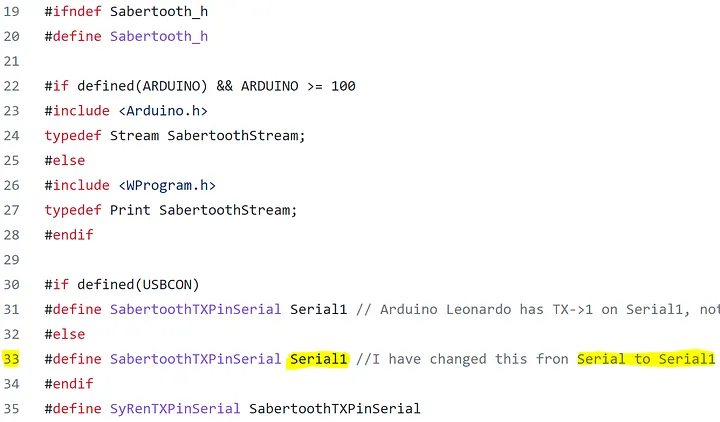
\includegraphics[width=0.72\linewidth]{figures/photos/sabertooth_serial1_article.png}
\caption{Firmware note from legacy assets: the Teensy uses a hardware serial port for Sabertooth communication while USB serial remains available to the NUC.}
\end{figure}

Current firmware files in the RUDRAv4 workspace are:

\begin{lstlisting}[caption={RUDRAv4 firmware locations.}]
src/rudra_base_bridge/firmware/uno_ps2_plain_serial/uno_ps2_plain_serial.ino
src/rudra_base_bridge/firmware/teensy_sabertooth_serial_controller/teensy_sabertooth_serial_controller.ino
src/rudra_base_bridge/firmware/teensy_sabertooth_imu_odom_controller/teensy_sabertooth_imu_odom_controller.ino
\end{lstlisting}

\section{Arduino Uno as the PS2 input controller}
The Uno keeps the PS2 receiver isolated from the main motor controller.  The current Uno packet is:

\begin{lstlisting}[caption={Uno to NUC joystick packet.}]
J,select,ry,rx,ly,lx,guard
\end{lstlisting}

The known PS2 receiver pin configuration from the RUDRA material is:

\begin{lstlisting}[language=C++,caption={PS2X receiver pin mapping.}]
ps2x.config_gamepad(9, 7, 6, 8, true, true);
// clock=9, command=7, attention=6, data=8
\end{lstlisting}

\begin{figure}[h]
\centering
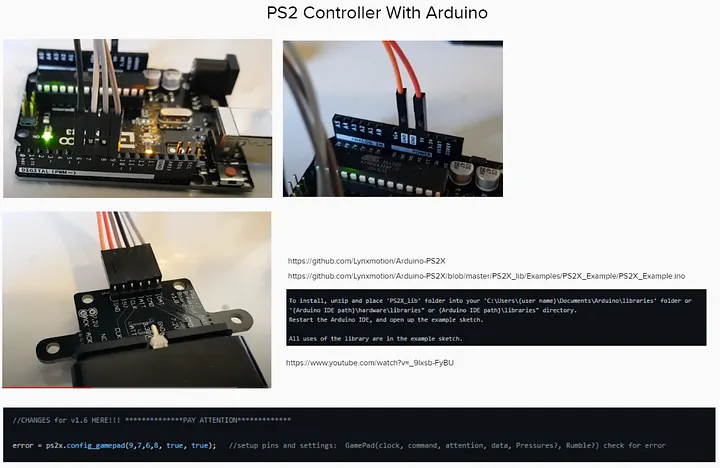
\includegraphics[width=0.92\linewidth]{figures/photos/ps2_controller_arduino_photo.png}
\caption{PS2 controller with Arduino reference image from the RUDRA article assets.}
\end{figure}

\section{Guard latch semantics}
The seventh Uno field, \cmd{guard}, is a latched obstacle-guard command.  Pressing \cmd{START} toggles the latch in the Uno firmware.  The ROS bridge follows that state and publishes \topic{/rudra/obstacle_guard}.  This means obstacle-guard enablement is observable in ROS rather than hidden in a controller sketch.

\section{Teensy command and acknowledgement contract}
The current manual drive path sends this line from the NUC to the Teensy:

\begin{lstlisting}[caption={NUC to Teensy drive packet.}]
D,left,right,enable
\end{lstlisting}

The Teensy replies with an acknowledgement line such as:

\begin{lstlisting}[caption={Teensy acknowledgement packet.}]
ACK,left,right,enable
\end{lstlisting}

For localization firmware, the Teensy also emits telemetry:

\begin{lstlisting}[caption={Teensy telemetry packet types.}]
IMU,ax,ay,az,gx,gy,gz
ODOM,x,y,theta,linear_x,angular_z,left_vel,right_vel
\end{lstlisting}

These packets are not a debug print afterthought.  They are the firmware-to-ROS contract.  Changing a field order in firmware must be matched by a change in the ROS parser and documented in the serial-protocol chapter.

\section{Firmware timing}
The Teensy should perform three timing-sensitive tasks even if ROS is temporarily delayed:

\begin{enumerate}
  \item Maintain a command watchdog.  If no valid command arrives within the timeout, write zero motor commands.
  \item Keep motor-output updates deterministic.  The Sabertooth bus is slow compared with internal MCU execution, so command scheduling must be simple.
  \item Keep encoder and IMU acquisition independent of Linux scheduling jitter.
\end{enumerate}

\begin{figure}[htbp]
\centering
\resizebox{0.90\linewidth}{!}{%
\begin{tikzpicture}[node distance=10mm and 14mm, every node/.append style={font=\small}]
  \node[rudraHw,text width=22mm] (ps2) {PS2\\receiver};
  \node[rudraBlock,text width=28mm,right=of ps2] (uno) {Arduino Uno\\\cmd{J,...}};
  \node[rudraBlock,text width=34mm,right=of uno] (nuc) {NUC ROS bridge\\topics and guard};
  \node[rudraBlock,text width=33mm,below=12mm of nuc] (teensy) {Teensy~4.1\\\cmd{D,...}, \cmd{ACK,...},\\IMU, ODOM};
  \node[rudraHw,text width=31mm,right=of teensy] (st) {Two Sabertooths};
  \draw[rudraArrow] (ps2) -- (uno);
  \draw[rudraArrow] (uno) -- node[above=0.5]{\scriptsize USB 115200} (nuc);
  \draw[rudraArrow] (nuc) -- node[left]{\scriptsize USB 115200} (teensy);
  \draw[rudraArrow] (teensy) -- node[above=0.75]{\scriptsize Serial1 9600} (st);
\end{tikzpicture}}
\caption{Microcontroller timing and ownership boundaries. The NUC supervises ROS-side behavior, while the Teensy remains the deterministic motor-control endpoint.}
\end{figure}

\section{Flashing workflow}
\begin{enumerate}
  \item Open the correct sketch in Arduino IDE or build it with Arduino CLI.
  \item Select the correct board: Uno for PS2 firmware, Teensy 4.1 for base firmware.
  \item Select the correct serial port.  Prefer \filep{/dev/serial/by-id} for runtime, but IDEs often display \filep{/dev/ttyACM*}.
  \item Upload the sketch.
  \item Close Serial Monitor before launching ROS.  Serial Monitor can hold the same port ROS needs.
  \item Run \cmd{bash scripts/list_serial.sh} again and update \filep{rudra_v4_hardware.yaml} if the by-id path changed.
\end{enumerate}

\section{Test ladder}
\begin{enumerate}
  \item Uno only: echo \topic{/rudra/ps2_raw}; sticks and SELECT should change.
  \item Teensy only: send neutral drive packets and expect \topic{/rudra/teensy_ack}.
  \item Teensy with wheels lifted: send low left/right commands.
  \item Full PS2 bridge with SELECT disabled: no wheel motion.
  \item Full PS2 bridge with SELECT enabled: low-speed manual motion.
  \item Kill the ROS launch while motors are spinning slowly: the Teensy watchdog must stop the motors.
\end{enumerate}
